\documentclass[journal,compsoc,10pt]{style/IEEEtran}
% \documentclass[10pt]{style/IEEETran}
% \usepackage{times}
% \usepackage{fullpage}
%% \usepackage{latex8}
\usepackage[pdftex]{graphicx}
\usepackage{subfig}
\usepackage[]{rotating}
\usepackage{url}
% \usepackage{comment}
\usepackage{amssymb}
\usepackage{amsmath}
\usepackage[usenames,dvipsnames]{color}
\usepackage{wrapfig}
\usepackage{epsfig}
% \usepackage{style/savetrees}
\usepackage{style/algorithm}
\usepackage{style/algorithmicx}
\usepackage{style/algpseudocode}
\usepackage{amsthm}
\usepackage{framed}
\usepackage{fancybox}
\usepackage{fancyhdr}
\usepackage{setspace}
\usepackage{xspace}
% \usepackage{tikz}
\usepackage{listings}
\usepackage{ifthen}
\usepackage{balance}
\usepackage{multirow}
\usepackage{caption}
\DeclareCaptionType{copyrightbox}

%conditional so I can compile with minted, others with lstlisting in case they
%don't have it
\newif\ifm
% \mfalse
\mtrue
\ifm
\usepackage{minted}
\usemintedstyle{friendly}
% \usemintedstyle{bw}
\fi

\setminted{frame=single}

\lstset{language=c}
\lstset{basicstyle=\scriptsize\ttfamily}
\lstset{keywordstyle=\color{blue}\bfseries}
\lstset{commentstyle=\ttfamily\color{ForestGreen}}
\lstset{frame=single,framerule=0.5pt}
\lstset{belowskip=\smallskipamount}
\lstset{aboveskip=\smallskipamount}
\lstset{showstringspaces=false}
% \lstset{morekeywords={kernel,reduce,__global__,out,float2,float4}}
% \pagestyle{plain}
% \pagenumbering{arabic}

\makeatletter
\newbox\sf@box
\newenvironment{SubFloat}[2][]%
{\def\sf@one{#1}%
  \def\sf@two{#2}%
  \setbox\sf@box\hbox
  \bgroup}%
{ \egroup
  \ifx\@empty\sf@two\@empty\relax
  \def\sf@two{\@empty}
  \fi
  \ifx\@empty\sf@one\@empty\relax
  \subfloat[\sf@two]{\box\sf@box}%
  \else
  \subfloat[\sf@one][\sf@two]{\box\sf@box}%
  \fi}
\makeatother

% \let\oldthebibliography=\thebibliography
% \let\endoldthebibliography=\endthebibliography
% \renewenvironment{thebibliography}[1]{%
% \begin{oldthebibliography}{#1}%
% \setlength{\parskip}{0.75ex}%
% \setlength{\itemsep}{0.75ex}%
% }%
% {%
% \end{oldthebibliography}%
% }

\IEEEoverridecommandlockouts

\begin{document}

\newcommand{\tsar}[0]{CoreTSAR\xspace}
\newcommand{\tsarlong}[0]{CoreTSAR\xspace(Task-Size Adapting Runtime)\xspace}
\newcommand{\ctsar}[0]{CoreTSAR\xspace}
\newcommand{\pgia}[0]{PGI Accelerator\xspace}

\newcommand{\tom}[1]{
  \begin{framed}
    \noindent{\color{ForestGreen}{\sc TOM:} \em #1}
  \end{framed}
}
\newcommand{\bronis}[1]{
  \begin{framed}
    \noindent{\textcolor{blue}{{\sc BRONIS:} \em #1}}
  \end{framed}
}
\newcommand{\tim}[1]{
  \begin{framed}
    \noindent{\textcolor{yellow}{{\sc TIM:} \em #1}}
  \end{framed}
}

\newcommand{\alex}[1]{
  \begin{framed}
    \noindent{\textcolor{red}{{\sc ALEX:} \em #1}}
  \end{framed}
}

\graphicspath{{pics/}}
% \authorinfo{author1 \and author2 \and author3 \and author4}
% {author's department\\
% location}
% \authorinfo{Thomas R. W. Scogland \and Wu-chun Feng }
% {Department of Computer Science, Virginia Tech, \\
% Blacksburg, VA 24060 USA}
% {\{tom.scogland,wfeng\}@vt.edu}
% \authorinfo{Barry Rountree \and Bronis R. de Supinski}
% {Center for Applied Scientific Computing, Lawrence Livermore National
% Laboratory,\\ Livermore, CA 94551 USA\\}
% {\{rountree,bronis\}@llnl.gov}


%% BRONIS: Looks like we are listing authors alphabetically
%% BRONIS: In that case, I go under 'd'; We could discuss
%% BRONIS: other orders and  Iwould probably be OK with them
\author{
 Bronis~R.~de~Supinski, Alejandro~Duran, Timothy~Mattson, 
 Thomas~R.~W.~Scogland,
}

\pdfinfo{
}

\title{
The Ongoing Evolution of OpenMP
}


\date{}
\maketitle

% \begin{IEEEkeywords}
% GPGPU; OpenMP; Programming models; Co-scheduling;
% \end{IEEEkeywords}

% \tom{need to update keywords}

\begin{abstract}

This paper presents an overview of the past, present and future
of the OpenMP Application Programming Interface (API). While the API
originally specified a small set of directives that guided shared 
memory fork-join parallelization of loops and coarse-grain program 
sections, OpenMP now provides a richer set of directives that capture
a wide range of parallelization strategies that are not strictly 
limited to shared memory. As we look towards the future of OpenMP,
we immediately see further evolution of the support for that range 
of parallelization strategies and the addition of direct support for 
debugging and performance analysis tools. Looking beyond the next 
major release of the specification of the OpenMP API, we expect the 
specification eventually to include support for more parallelization
strategies and to embrace closer integration into its Fortran, C and,
in particular, C++ base languages, which will likely require the 
API to adopt additional programming abstractions.

\end{abstract}

\section{Introduction}
\label{sec:intro}

The OpenMP effort began in 1996 when a handful of vendors (DEC, HP, IBM, Intel,
Kuck and Associates, and SGI) were brought together by the Accelerated Strategic
Computing Initiative~(ASCI) of the Department of Energy~(DOE) to create a
portable application programming interface~(API) for shared memory computers
based on their various implementations of, and extensions to, the Parallel
Computing Forum directives~\cite{TheParallelComputingForum}. Vendors do not
typically work well together unless an outside force compels cooperation. Mary
Zosel and the ASCI parallel tools team provided that compulsion by communicating
that ASCI would only purchase systems with a portable API for shared memory
programming. Their role in the beginning of OpenMP ensured that it met the needs
of HPC applications programmers.

Early public presentations about the project~\cite{ewomp99} clearly
defined the initial group's goals:
%The OpenMP Architecture Review Board and the future of OpenMP, Tim Mattson,
%European Workshop on OpenMP, Lund, Sweden, September 30 - October 1, 1999

\begin{itemize}
  \item To support portable, efficient and comprehensible shared-memory 
        parallel programs;
  \item To produce specifications based on common practice that 
        could be readily implemented;
  \item To provide a consistent API for Fortran, C and C++ to the 
        most reasonable extent possible;
  \item To be lean and mean, i.e., to  be only as large as required 
        to express important control-parallel, shared-memory programs  
        but no larger;
  \item To ensure API versions are backwards compatible;
  \item To support \emph{serial equivalence}, i.e., for it to be possible to
    write OpenMP programs to produce the same result whether run serially or in
        parallel, to the greatest possible extent.
\end{itemize}

The first OpenMP specification  was released in November 1997 at SC97. The
early OpenMP community knew that other parallel programming  standardization 
efforts, such as HPF~(High Performance Fortran) and MPI 2.0, suffered from 
multi-year delays as implementors struggled to produce robust, 
application-ready implementations. Thus, OpenMP by design narrowly focused 
on current practice. This focus led to the availability of multiple
vendor-supported implementations within a year of the release of the 
first specification. 

\begin{figure}
\begin{minted}{c}
#pragma omp parallel // fork
{
  // share the loop across threads,
  // reducing into total
  #pragma omp for reduction(+:total)
  for (int i=0; i<N; ++i) {
    total += foo(i);
  }
} // join
\end{minted}
\caption{Basic OpenMP\label{fig:basic}}
\end{figure}

Over time, additional vendors and research organizations joined the effort.  A
non-profit corporation, the OpenMP Architecture Review Board~(ARB), was created
to prevent any single vendor from dominating the standard. The current 30
members of the OpenMP ARB continue to own and to evolve the API to serve the
needs of parallel application programmers. The ARB retains many of the original
goals in its current mission, which is to standardize directive-based
multi-language high-level parallelism that is performant, productive and
portable. The OpenMP API now provides a portable, scalable model that gives
parallel programmers a simple and flexible interface for developing parallel
applications for platforms ranging from embedded systems and accelerator
devices to multicore systems.  A simple example of the iconic workshared
parallel for loop is shown in Figure~\ref{fig:basic}, showing the basic
fork-join model of parallel with a workshared loop and a reduction in OpenMP
syntax that has been valid from the first release of the C version of the
specification until today.

OpenMP retains all but two of its original goals. Specifically, OpenMP has 
evolved to support almost all parallel programming patterns, which necessarily
implies a larger specification than originally envisioned. Further, while 
serial equivalence is still achievable, that range of patterns necessarily 
leads to many opportunities to deviate from it. Otherwise, the only change 
to the original goals is that the scope of OpenMP has extended beyond 
shared memory. 

We comprehensively examine the state of OpenMP in anticipation of the imminent 
release of version 5.0 of the API. We first review the evolution of OpenMP 
through version 4.5 (Section~\ref{sec:evolve}). We then provide a more 
detailed examination of the philosophy that has guided its evolution 
(Section~\ref{sec:philosophy}). Next, we briefly review the basic concepts 
and mechanisms that support implementation of the evolving API 
(Section~\ref{sec:concepts}). We then detail some recent 
(Section~\ref{sec:recent_extensions}) and impending 
(Section~\ref{sec:in_progress}) additions to OpenMP. Finally, we discuss
and anticipate some possible directions for its longer term evolution
(Section~\ref{sec:future_directions}).

\section{An Overview of OpenMP's Evolution}
\label{sec:evolve}

OpenMP is a living language that reflects the needs of its many users. 
As hardware capabilities and the range of supported algorithms have 
grown, the complexity of the specification has also expanded. 
Figure~\ref{omppcount} lists the number of pages of the versions of 
the specification (not including front matter, appendices or indices).   
The initial OpenMP specification~\cite{openmp1f} (OpenMP Version 1.0 for
Fortran) was 40 pages long. The latest specification~\cite{openmp45} (OpenMP 4.5
for Fortran, C and C++) is 303 pages long.

Figure~\ref{omppcount} also details the evolution of language support.
Prior to the release of version 2.5~\cite{openmp25} in 2005, each OpenMP specification 
was specialized to a particular language (i.e., to Fortran or to C and 
C++). This division simplified writing the text of the specification, 
but also created difficulties. First, most of the people working on the 
Fortran specifications also worked on the C/C++ specifications. Thus, the 
evolution of the API was hampered since we could not run the two 
language committees in parallel. Thus, updates to the specification 
were produced slowly relative to the amount of new material in them. For
example, OpenMP 2.0 for C/C++~\cite{openmp2c} (50 pages) was released almost 4
years after OpenMP 1.0 for C/C++~\cite{openmp1c} (45 pages) despite the
relatively simple extensions that it included. 

Not only was the progress of the API slower due to the separate 
specifications, the separation also allowed the API to have subtle 
differences across the languages. The process of merging the separate
APIs for the languages into a single  specification was a much larger 
undertaking than any of us expected. That process required us to recast 
OpenMP's core abstractions much more carefully so they would apply across 
the languages. The resulting OpenMP version 2.5 specification (117 pages)
took three years to create despite adding few new capabilities.

Following the merger of the specifications and the growth in the popularity
of the API, as evidenced by the expanding membership of the OpenMP ARB,
the pace of the evolution of OpenMP has increased. Today, OpenMP is no 
longer a simple API for which its full breadth can be learned in less 
than a day. Nonetheless, the core features of the version 1.0 specifications
remain and the goal of backwards compatibility has largely been achieved.

The OpenMP version 3.0 API specification~\cite{openmp3} (151 pages) added
task-based parallelism. This addition supports irregular parallelism, unlike the
loop-based constructs of the previous specifications. OpenMP 3.0 also provided
much more control over the existing support for structured parallelism. OpenMP
version 3.1~\cite{openmp31} (160 pages) extended the support for structured parallelism, for
example, by adding straightforward control of the number of threads used at each
level of nested parallelism. OpenMP 3.1 also further refined tasking support. In
general, the continued evolution of OpenMP has advanced the original features
while also expanding the types of parallel algorithms that the specification
supports.

The OpenMP version 4.0 API specification~\cite{openmp4} (248 pages) added support for 
accelerator-based systems through its device constructs. Echoing the API's 
original purpose, OpenMP 4.0 also standardized directives for SIMD 
parallelism, which had become widely supported by many compilers but 
with subtly different semantics. OpenMP 4.5~\cite{openmp45} (303 pages) added many 
refinements to those addition and elsewhere. As we later discuss in 
detail, OpenMP 5.0 will support mechanisms to control data placement in
complex, multi-level memory systems. It will also include support for
first-party and third-party tools as well as the customary major 
extensions for the types of parallelism already supported by OpenMP.

In evolving the OpenMP API, we have added features that address 
non-uniform memory architectures, more complex concurrency control, 
irregular algorithms, accelerators, and much more. The specification 
has not grown due to a lack of discipline in its designers. Instead,
its growth reflects user demands for new features and how hardware 
has changed. In that light, a 7.5X increase in size over the course 
of almost 20 years is not surprising.

\begin{figure}
  \centering
  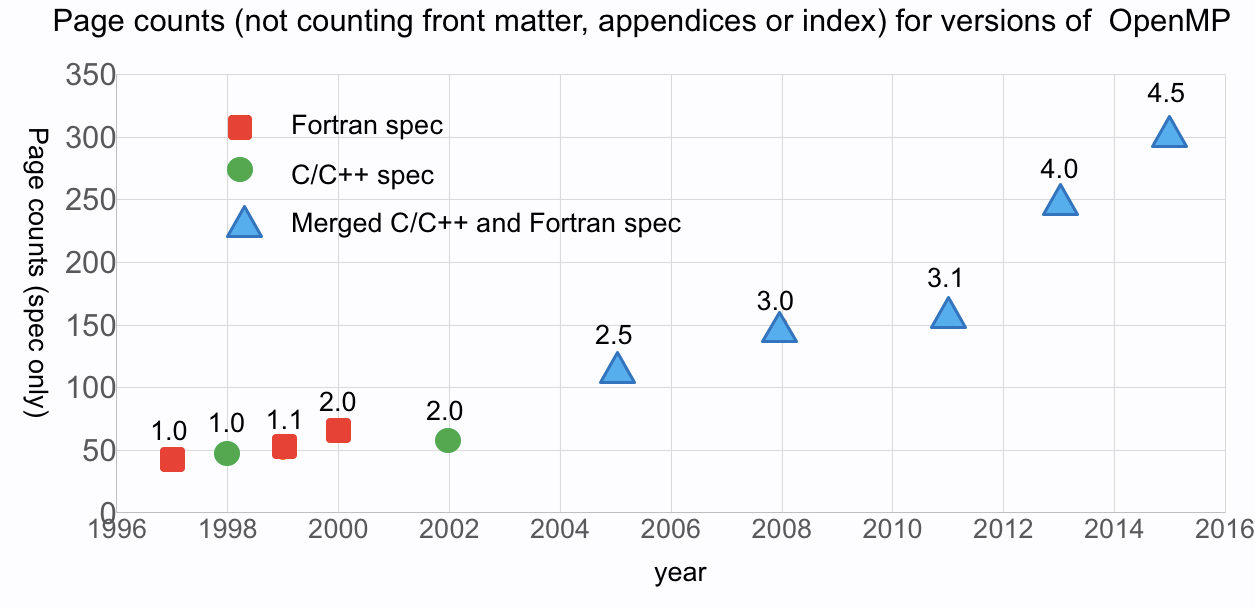
\includegraphics[width=3.4in]{pics/opcounts.png}
  \caption{OpenMP Specification Growth Across Versions}
  \label{omppcount}
\end{figure}



\section{The Guiding Philosophy of OpenMP}
\label{sec:philosophy}

The general philosophy of OpenMP reflects the ARB's mission to standardize 
directive-based multi-language high-level parallelism that is performant, 
productive and portable. Portability is achieved first and foremost through
broad adoption and support of the specification. At the highest level, a 
directive-based approach supports productivity through incremental 
parallelization and refinement through which user code remains as close 
to its original serial version as possible while still achieving performance 
goals. Directives allow the programmer to specify information that a compiler
would otherwise not be able to determine -- or that might require complex
and error-prone analysis. Further, OpenMP provides sensible defaults that 
often result in high performance but also allows low-level control of 
aspects that the compiler and runtime may not deduce high quality settings.

As we discussed in the introduction, OpenMP retains many of its original
goals, which embodied a general philosophy. However, like the specification, 
the philosophy of OpenMP has evolved as it has expanded to support a wider
range of parallel programming patterns. The remainder of this section 
discusses the evolution of two key aspects of the original philosophy,
language independence and serial equivalence, as well as the issue of
descriptiveness versus prescriptiveness, a philosophical issue for 
programming models that has recently received significant attention.

\subsection{Relationship to Base Languages}
\label{sub:relationship_to_base_languages}

Although OpenMP began with separate specifications for C/C++ and 
Fortran, as we discussed in Section~\ref{sec:evolve}, OpenMP 2.5 
merged them into a single document. Although that choice was
partly due to the pragmatic reduction in effort to move the base 
languages forward together, the original goal of a consistent API 
across the base languages, which remains a key part of OpenMP's 
guiding philosophy, was the most important reason. This language 
independence is one of OpenMP's core strengths since OpenMP has 
greater portability and generality, not only across the C, C++ 
and Fortran base languages but also in its design as a result. 

%% BRONIS: My solution is to merge the two sections since
%% BRONIS: language independence is just one aspect of the
%% BRONIS: relationship to the base language
%% \tom{this is too short, ideas on how to expand?}

%% BRONIS: Still need to rework the following paragraph
%% BRONIS: Need to introduce the concept of directives
%% BRONIS: being Turing complete and that OpenMP can bridge
%% BRONIS: differences across the languages

OpenMP, by itself, is not a language.  It provides an API for expressing
parallelism and concurrency in a portable way across three independent
languages, with the goal of providing the same experience and easy
interoperability between all three.  Because of this it relies heavily on each
base language to define the behavior of a given construct within each thread of
execution or block of code.  The relationship with the base languages has
changed somewhat over time however.  Before the release of C11 and C++11, C and
C++ themselves had no well-defined concept of a data race, or of threading in
general.  In fact, the ISO C99 standard~\cite{c99} does not contain the word
"thread" at all, and contains the word "race" only as part of the word "brace."
As a result, OpenMP has to provide all threading and memory model semantics for
a program written using OpenMP constructs in the context of a C99 program.  With
the advent of integrated threading models, acquire and release memory models and
more built-in parallel concepts OpenMP is now in a position of providing its own
semantics in the context of those models and integrating with them.



\subsection{Serial Equivalence}
\label{sub:serial_equivalence}

A original goal for OpenMP was to support serial equivalence to the 
greatest possible extent. As a result, many think that all OpenMP programs, 
or at least all correct OpenMP programs, are guaranteed the same result
if the code is executed in parallel as when the compiler completely 
ignores all OpenMP constructs. However, even OpenMP 1.0 included runtime
functions that allow a program to depend on the number of threads or the
thread number (or ID) that executed a region. Thus, trivial programs could
fail to exhibit serial equivalence. Today, many more opportunities exist
to write OpenMP programs that do not provide serial equivalence. 
%% BRONIS:Could include the trivial example here

%% BRONIS: Tom, you mentioned data privatization in the text that I
%% BRONIS: deleted. Do you have an interesting example in mind?

As OpenMP has evolved, the opportunities to write programs that do not
exhibit serial equivalence have increased. OpenMP support for tasking 
provides numerous opportunities. Figure~\ref{fig:trivial_task} provides
a simple tasking program in which the serial version has an infinite loop
while the parallel version will complete quickly, assuming that the parallel
region uses two or more threads and different threads execute the two tasks.
Figure~\ref{fig:trivial_target} shows a pair of example functions, where
\texttt{increment} will take and increment a value whether it executes with
OpenMP or not, \texttt{example} may or may not depending on the platform even
though it calls \texttt{increment} to do the work.  While this example clearly
contains a bug, such manipulations of device data lifetimes can cause different
execution between OpenMP and serial \emph{even when the OpenMP code is also
serial}.

\begin{figure}
\begin{minted}{c}
void example() {
  int a = 0;
  #pragma omp parallel
  {
    #pragma omp single
    {
      int b = 0;
      #pragma task
      while (b == 0) {
        #pragma atomic read seq_cst
        b = a;
      }
      #pragma task
      {
        #pragma atomic update seq_cst
        a++;
      }
    }
  }
}
\end{minted}
\caption{A trivial program with OpenMP tasking.\label{fig:trivial_task}}
\end{figure}

\begin{figure}
\begin{minted}{c}
void increment(int * p) {
  #pragma omp target map(tofrom:p[0:1])
  {
    (*p)++;
  }
}
void example() {
  #pragma omp target data map(to: p[0:1])
  example1();
}
\end{minted}
\caption{A trivial program with OpenMP target.\label{fig:trivial_target}}
\end{figure}

In general, serial equivalence requires the program or runtime to limit
the possible execution orders. As OpenMP has grown to support more parallel 
programming patterns, the range of execution orders has as well, which 
implies either more opportunities to eschew serial equivalence or more
limitations on the range of execution orders. Since such limitations would 
also create performance limitations, OpenMP (or any parallel programming 
system) tries to avoid them unless the programmer requires them. Thus, the 
philosophy of OpenMP remains to provide constructs that simplify the 
enforcement of serial equivalence when desired but that has evolved not 
to limit parallelism -- and by extension -- performance unnecessarily.


\subsection{Descriptive or Prescriptive Semantics}
\label{sub:descriptive}

The high performance community is currently debating the value of 
\emph{descriptive} versus \emph{prescriptive} programming semantics. 
Semantics are descriptive if programming constructs describe the 
computation that should be performed but provide the compiler and 
runtime the flexibility to determine exactly how to perform the 
computation. Programming constructs with prescriptive semantics 
prescribe all details of how to perform the required computation.

Our position is that the debate is misguided since it assumes a binary 
choice between the two types of semantics. However, almost all languages 
have constructs that are descriptive while others are (more) prescriptive. 
Specifically within the HPC community, some claim that OpenACC is descriptive 
while OpenMP is prescriptive~\cite{juckeland2016isc,wolfe16descriptive}. 
While OpenACC provides more descriptive constructs in its most recent version 
than OpenMP does, the \texttt{acc parallel loop} directive is prescriptive 
since sometimes users want to \emph{prescribe} that a loop must be parallelized. 

Alternatively, most OpenMP defaults allow the compiler freedom
to choose details about how the computation is performed. Even
the \texttt{num\_threads} clause of the \texttt{parallel} construct,
which many believe to be among its most prescriptive mechanisms,
allows the compiler and runtime to determine if the number of
threads requested are available. If that many threads are not
available, the compiler and runtime have the flexibility to
determine how many threads to use. So, one may see the issue 
as where to place a language, or even its constructs, on a 
continuum of possible semantics.

More importantly, choosing one place on that continuum is overly
limited and fails to address the overall preference of programmers. 
Specifically, they would prefer that the compiler and runtime would 
always ``do the right thing'' given a description of the computation 
to perform. However, in reality, compilers and runtimes often do not. 
In these instances, programmers prefer to have the ability to override 
their decisions and to prescribe exactly how to perform the computation.

For these reasons, the emerging OpenMP philosophy is to provide
mechanisms that describe the computation to perform and that
prescribe as much or as little as the programmer desires about
how to perform it. As a first step, OpenMP 5.0 will add the 
\texttt{loop} construct, which only informs the compiler 
and runtime that a loop nest is easily parallelized. In the 
longer run, we are exploring mechanisms that specify that the 
intent of a clause or a construct is fully descriptive or prescriptive.


\section{Concepts and Mechanics}
\label{sec:concepts}

OpenMP has expanded greatly in scope and complexity since its inception, but
many of the features build on a common set of core mechanics and basic concepts
that have changed relatively little over the past twenty years.  This section
describes two of the most important building blocks of OpenMP, outlining and
data environments.

\subsection{Outlining}
\label{sub:outlining}

Outlining is the opposite of inlining, extracting a function from the body
of another function.  In the context of OpenMP, compiler outlining forms the
basis of many of the features that allow OpenMP directives to parallelize what
otherwise looks like normal serial code by automatically creating the functions
required as targets for the underlying operating system's threading primitives.
By way of an example, an implementation might convert a parallel region like
the one in Figure~\ref{fig:outline-before} into a new function and a call, or
calls, into the runtime as in Figure~\ref{fig:outline-after}.

\begin{figure}
\begin{minted}{c}
void foo () {
  int a;
  #pragma omp parallel
  {
    #pragma omp master
    a = omp_get_num_threads();
  }
}
\end{minted}
\caption{A function using OpenMP before outlining is applied}
\label{fig:outline-before}
\end{figure}

\begin{figure}
\begin{minted}{c}
struct foo_parallel_0 {
  int *a;
};
void foo_parallel__(void *data_in) {
  struct foo_parallel_0 * data = data_in;
  data->a[0] = omp_get_num_threads();
}
void foo () {
  int a;
  struct foo_parallel_0 data = {&a};
  runtime_parallel(foo_parallel__, &data);
}
\end{minted}
\caption{After outlining is applied}
\label{fig:outline-after}
\end{figure}

This example is substantially simplified, but the general transformation for
outlining any block is to generate a structure that holds all necessary state
and a function with a signature compatible with the threading abstraction in
use.  The end result is that the user doesn't have to deal with manually
creating wrapper functions and single-use structures to encapsulate their code
whenever something should be run in parallel or made into a task, the compiler
can do that for them.

In fact, it could be argued that the main reason that OpenMP was created as a
compiler extension rather than as a library is to leverage the compiler's
ability to outline regions of code.  Languages like C++11 and C with the blocks
extension can cover many of OpenMP's original features, though not some of the
new ones, by using the lambda or block construct of the language to provide
outlining at the user level.  We'll revisit this in
Section~\ref{sec:future_directions} when we discuss some of the ways OpenMP is
planning to grow in the future.

\subsection{Data Environments}
\label{sub:data_environments}

While outlining provides the transformation necessary to allow code to remain
written in a serial style, it doesn't directly address the issue of data privacy
between threads or tasks.  In OpenMP, every task, or implicit task as used by
constructs like \texttt{for} and \texttt{simd}, has its own data environment
that represents its view of memory and of state in the OpenMP runtime.  The
simplest manifestations of the data environment are providing variables that are
private to the task, thread, team or construct in general without having to
re-factor the declaration and initialization of such variables in user code.

A less known but equally important property is the handling of OpenMP
ICVs~(Internal Control Variables).  Most users know some of the major ICVs by
their associated environment variables, like \texttt{OMP\_NUM\_THREADS} for
example, and in fact the behavior of environment variables and data environments
are relatively similar.  Each new data environment inherits the values or
behaviors of the enclosing data environment, but is henceforth independent of
the enclosing environment.  This allows each task to control the behavior of
OpenMP in its own dynamic scope without changing the behavior of OpenMP
constructs outside of that scope, giving the user more composability and
control.


\section{Recent OpenMP Extensions}
\label{sec:recent_extensions}

OpenMP 4.0 extends the API to cover two additional major forms of
parallelism: accelerator offload and SIMD vectorization. Almost all
current systems include hardware that require these parallel programming 
patterns. This section discusses the related extensions as well as several 
tasking extensions in OpenMP 4.0 and 4.5.

\subsection{SIMD}
\label{sub:simd}

Compilers have included technology to auto-vectorize loops for many years. 
However, this support has limited effectiveness for real applications because 
of the complexity of determining the potential correctness and benefit of 
vectorization (e.g., are loop iterations free of dependences). These 
limitations led almost all major compilers to include implementation-defined 
vectorization directives. While frequently spelled\texttt{ivdep}, the
semantics often subtly varied across compilers. Due to the similarity 
with the original motivation for OpenMP with respect to threading 
directives, we included explicit directives to exploit SIMD parallelism 
in OpenMP 4.0.

The \texttt{simd} directive expresses that a given loop nest has no
dependences that would prevent vectorization. The compiler can then 
vectorize the loop without performing any dependence analysis. The 
directive accepts several clauses that provide further information 
and/or restrictions to guide vectorization. The \texttt{simd} directive 
is not prescriptive as the compiler may choose not to vectorize the 
loop (essentially a vector width of one).

Loops with functions pose a particular problem to vectorization. If the 
compiler has the function definition available then it could inline it 
to vectorize the loop fully. In practice, the definition is often in a
different compilation unit. Without special treatment, the compiler can
still partially vectorize the loops by repeatedly calling the scalar 
function for each element of the vector. A more efficient solution 
generates vector variants of the functions that process multiple 
elements of the vector in a single invocation. The compiler can then
use these variants in loops annotated with the \texttt{simd} directive.

OpenMP provides the \texttt{declare simd} directive to guide generation
of vector function variants. The directive accepts several clauses that
prescribe generation of efficient variants for specific use cases so a
function may be annotated with multiple \texttt{declare simd} directives.
Other clauses generally guide generation of vector variants (e.g., the 
\texttt{uniform} clause indicates that a given argument should be a 
scalar and not a vector). The compiler can also generate other variants 
that may be useful for a specific target architecture. The simple example 
in Figure~\ref{fig:simd-example} uses the OpenMP SIMD directives.

\begin{figure}
\begin{minted}{c}

#pragma omp declare simd uniform(c)
double scale(double v, double c) {
     return v * c;
}

void example(double * v, size_t n) {
    double alpha = 0.5;
#pragma omp simd
    for (size_t i = 0; i < n; i++ )
        v[i] = scale(v[i], alpha);
}
\end{minted}
\caption{OpenMP SIMD Vectorization Example\label{fig:simd-example}}
\end{figure}





\subsection{Devices}
\label{sub:devices}

In addition to the pervasiveness of vector units in modern processors, many
systems now include additional co-processors or computational accelerators.  
These devices include hardware such as Graphics Processing Units~(GPUs), 
Digital Signal Processors~(DSPs), and computation offload co-processors 
like the Intel Xeon Phi. While these hardware devices usually reside in 
a single node, they pose a particular challenge for OpenMP because they 
frequently use a different instruction set and programming paradigm. Further,
they often do not coherently share memory with the host processors that
OpenMP originally targeted.

OpenMP~4.0 added the \texttt{target} directive and related directives and 
routines to address these devices. These additions provide an offload model
that uses the existing shared-memory model on each device. Since many 
accelerators are many-core devices, we added the \texttt{teams} and 
\texttt{distribute} directives, which create leagues of independent thread 
teams and share loop iterations among them. Accelerators can execute these 
teams efficiently since synchronization across them is highly restricted while
all OpenMP functionality (except the device constructs) may be used within 
each team. The code in Figure~\ref{fig:target-loop} offloads a simple loop 
to the default device and divides its work across teams of threads. The 
\texttt{map} clauses map data into the device data environment and, if 
desired, update the view of the data on the device (host) before (after)
execution of the \texttt{target} region.

\begin{figure}
\begin{minted}{c}
#pragma omp target teams distribute \
            parallel for            \
            map(to: in_arr[0:n])    \
            map(from: out_arr[0:n])
for(size_t i = 0; i < n; ++i)
  out_arr[i] = in_arr[i] * in_arr[i];
\end{minted}
\caption{OpenMP Device Offload Example\label{fig:target-loop}}
\end{figure}

In addition to the \texttt{map} clause on the \texttt{target} directive, 
OpenMP provides several other options for device data management. These 
options include directives for the definition of structured target data 
regions and also for unstructured transfers or updates between host and 
device data. The \texttt{nowait} clause can be used on the \texttt{target}
directive and on these device data management directives to enable the 
implementation to treat them as asynchronous tasks. This feature allows 
overlap of host and device computation and data transfers. It can also be 
combined with task dependences, described in Section~\ref{sub:tasking}, for 
data-driven asynchronous execution. 
%% BRONIS: Seems like a throwaway line since we do not say anything about them
%% Device memory runtime routines are also provided.

Similarly to \texttt{simd} regions, \texttt{target} regions that contain 
function calls are particularly challenging to support.  Unlike with 
\texttt{simd} regions, however, if the function definition is not 
available to the compiler then the compiler may not generate any variant
that can be executed, even inefficiently, on the device. Thus, in OpenMP 4.0
and 4.5, if any target region calls a function then the user must annotate  
the function definition and its declarations with the \texttt{declare target} 
directive. The directive can also be applied to global variables. The compiler
then must generate a variant of a function or a static lifetime variable for 
the target device. 


\subsection{Tasking Extensions}
\label{sub:tasking}

%% BRONIS: We should  cover 4.0 and 4.5 tasking extensions
%% BRONIS: Specifically: Discuss task dependences, taskgroup and taskloop

%% STEPHEN: Introduce the problem with OpenMP 3.x

Directives to support asynchronous task parallelism were first introduced in OpenMP 3.0, and the initial design rationale for this capability is explained in an article by Ayguad\'{e} et al.~\cite{ayguade2009tpds}.  Along with task generation using the \texttt{task} construct, task synchronization is provided using the \texttt{taskwait} construct and barriers.  The \texttt{taskwait} construct specifies a wait on the completion of child tasks of the current task, and a barrier requires complete execution of all tasks in the current parallel region before any threads in the team are allowed to continue execution beyond the barrier.  In many instances, these simple synchronization mechanisms lack the expressiveness to fully expose all available application parallelism.  OpenMP 4 addresses such limitations with two additional synchronization mechanisms, task dependences and task groups.


%% SMATEO: this is a bit ugly, but it's the only way I know to do it :D
\begin{figure}

\newsavebox{\firstExample}
\newsavebox{\secondExample}

\begin{lrbox}{\firstExample}
%\begin{minipage}{0.48\columnwidth}
\begin{minipage}{0.45\columnwidth}
%\begin{minted}[fontsize=\small]{c}
\begin{minted}{c}
#pragma omp task
produce(a);
#pragma omp task
produce(b);
#pragma omp task
produce(c);

// wait on all
//    three child
//    tasks here
#pragma omp \
        taskwait

#pragma omp task
consume(a, b);
#pragma omp task
consume(b, c);
#pragma omp task
consume(a, c);
\end{minted}
\end{minipage}
\end{lrbox}

\begin{lrbox}{\secondExample}
%\begin{minipage}{0.48\columnwidth}
\begin{minipage}{0.50\columnwidth}
%\begin{minted}[fontsize=\small]{c}
\begin{minted}{c}
#pragma omp task \
    depend(out: a)
produce(a);
#pragma omp task \
    depend(out: b)
produce(b);
#pragma omp task \
    depend(out: c)
produce(c);

#pragma omp task \
   depend(in: a, b)
consume(a, b);
#pragma omp task \
   depend(in: b, c)
consume(b, c);
#pragma omp task \
   depend(in: a, c)
consume(a, c);
\end{minted}
\end{minipage}
\end{lrbox}



\subfloat[][OpenMP 3.0]{\usebox{\firstExample}\label{fig:CodeTaskDeps3.0code}}
~
~
\subfloat[][OpenMP 4.0]{\usebox{\secondExample}\label{fig:CodeTaskDeps4.0code}}

\centering{\subfloat{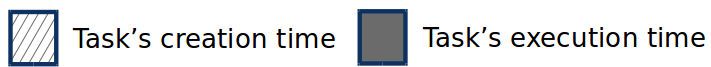
\includegraphics[width=0.30\columnwidth]{pics/intro_tasking_ex1_legend.png}}}
\addtocounter{subfigure}{-1}

\subfloat[][]{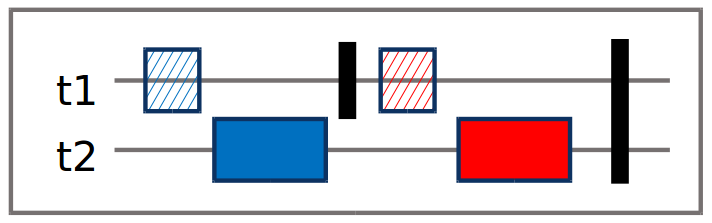
\includegraphics[width=0.48\columnwidth]{pics/intro_tasking_ex1_omp3.png}\label{fig:CodeTaskDeps3.0timeline}}
~
~
\subfloat[][]{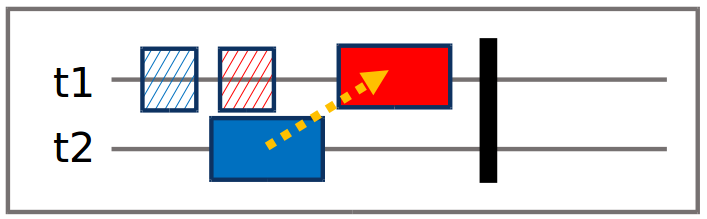
\includegraphics[width=0.48\columnwidth]{pics/intro_tasking_ex1_omp4.png}\label{fig:CodeTaskDeps4.0timeline}}
\caption{Tasking examples with and without dependences.\label{fig:CodeTaskDeps}}
\end{figure}

%% STEPHEN: Explain task dependences (with example, space permitting)

The \texttt{depend} clause was introduced in OpenMP 4.0 to indicate which variables are inputs and outputs of particular tasks, allowing the implementation to derive and resolve the data dependences between the tasks.  Figures~\ref{fig:CodeTaskDeps4.0code}~and~\ref{fig:CodeTaskDeps4.0code} show code for a producer-consumer pattern using tasks in OpenMP~3.0 and OpenMP~4.0, respectively.  The timelines below it illustrate the scheduling of the tasks onto two threads:  The exploitation of fine-grained, data-driven sychronization provided by task dependences, shown in Figure~\ref{fig:CodeTaskDeps4.0timeline}, allows more flexible scheduling compared to the more coarse-grained synchronization using OpenMP~3.0, shown in Figure~\ref{fig:CodeTaskDeps3.0timeline}.

%% STEPHEN: Sergi to provide performance results
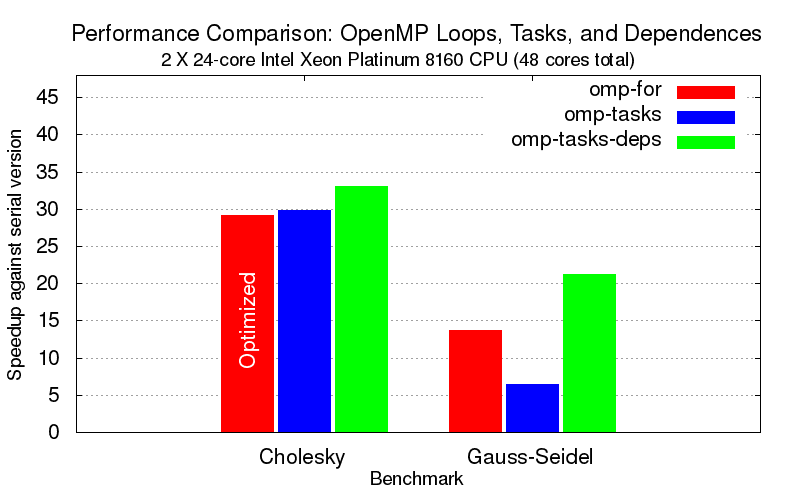
\includegraphics[width=0.45\textwidth]{pics/task-perf-results.png}

%% STEPHEN: Discuss task group (example needed or not?)

Recall that all child tasks of the current task must compete at a \texttt{taskwait} construct.  The \texttt{taskgroup} construct allows the current task to wait on only subset of its child tasks, while other child tasks may continue executing beyond the synchronization point.  Additionally, the current task waits on all descendant tasks of the child tasks in the task group, a behavior that may be termed deep synchronization.  Because child tasks of the current task can be excluded from a task group, those tasks could perform long-running background activities that proceed alongside successive computational kernels.


%% STEPHEN: Mention task priorities briefly?

% Michael: the subsubsection is just for my orientation and can be removed.
%\subsubsection{Taskloop}
\label{sec:Taskloop}

The task-based loop, or \emph{taskloop}, is an OpenMP~4.0 extension that enables composition of the tasking model with loop-based parallelism.
Since OpenMP~3.0, the programmer could manually decompose a loop into chunks and assign each chunk to an OpenMP task, but this code transformation was cumbersome and error-prone.
The \code{taskloop} construct automatically transforms a loop into a parallel loop executed using OpenMP tasks.

\begin{figure}
\begin{minted}{c}
void sapxy_tasks(float* a, float* b,
                 float s, size_t n) {
#pragma omp taskloop simd \
            num_tasks(NTASKS) \
            shared(a,b) firstprivate(s)
  for (size_t i = 0; i < n; i++) {
    a[i] = a[i] * b[i] * s;
  }
}
\end{minted}
\caption{Example for using the \code{taskloop} construct.\label{fig:TaskloopExample}}
\end{figure}

Figure~\ref{fig:TaskloopExample} shows the parallelization of a \emph{saxpy} operation using the \code{taskloop} construct.
The \code{num\_tasks} clause specifies the number of OpenMP tasks to create for the sapxy loop.
Alternatively, programmers can use the \code{grainsize} clause to specify the minimum number of loop iterations per task.
The \code{taskloop} construct is also available as a combined construct to use SIMD instructions within the generated tasks.

\subsection{Cancellation}
\label{sec:Cancellation}
OpenMP~4.0 introduced the concept of cancellation, a capability to end 
OpenMP regions \emph{early}. This capability enables efficient error
handling but also supports more efficient search algorithms. When a thread
encounters a \texttt{cancel} construct, it cancels execution of the 
inner-most associated region (as indicated by a \texttt{parallel}, 
\texttt{sections}, \texttt{for} or \texttt{do} clause) or associated set 
of tasks (as indicated by the \texttt{taskgroup} clause). 

Cancellation must occur with well-defined semantics so users can ensure 
that their data is in an expected state. Since the user can manage the 
state immediately before the \texttt{cancel} construct, the thread 
that encounters it immediately proceeds to the end of the canceled region 
(e.g., the end of the current task for the \texttt{taskgroup} clause). Other
threads must encounter a \emph{cancellation point}, prior to which the user 
can manage state, in order to process the cancellation. Cancellation points 
are implied at barriers and are explicitly indicated by a 
\texttt{cancellation point} or \texttt{cancel} construct. If a thread observes 
that another thread has canceled the associated region at a cancellation point,
it also proceeds to the end of the canceled region (e.g., the end of the 
current task). With the \texttt{taskgroup} clause, tasks that have not begun
to execute are simply discarded since they cannot have state from partial 
execution.

Figure~\ref{fig:Cancellation} shows how to cancel a binary tree search when 
the value is found. Without the OpenMP directives, the code recursively 
examines children nodes and stops if the value of the current tree node 
matches the search value. With OpenMP tasking, the subtree searches execute
in parallel. Without cancellation, once a tasks find search value, it will 
not generate any more tasks but the other branches of the parallel search 
will continue. With cancellation, any executing tasks will complete their 
check but any generated tasks that have not begun execution (including those 
generated by those executing tasks) are discarded so that unnecessary work 
is greatly reduced while still executing the search in parallel.

\begin{figure}
\begin{minted}{c}
bin_tree_t *
search_tree(bin_tree_t * tree, int val) {
  bin_tree_t * found = NULL;
  if (tree) {
    if (tree->val == val)
      found = tree;
    else {
#pragma omp task shared(found)
      {
        bin_tree_t * found_left =
          search_tree(tree->left, val);
        if (found_left) {
#pragma omp atomic write
          found = found_left;
#pragma omp cancel taskgroup
        }
      }
#pragma omp task shared(found)
      {
        // similar code for right branch
      }
#pragma omp taskwait
    }
  }
  return found;
}
\end{minted}
\caption{Cancellation Example\label{fig:Cancellation}}
\end{figure}





\section{The Next Evolutionary Step}
\label{sec:in_progress}

We will release OpenMP 5.0 in November 2018. We have already made 
substsantial progress on its content, as TR6~\cite{TR6} demonstrates.
Based on TR6, OpenMP 5.0 will increase the page count of specification 
more than any previous version. However, a large portion of the new
pages will detail additions to OpenMP that support performance analysis
and debugging tools; we will not detail those extensions. Nonetheless,
OpenMP 5.0 will also include several extensions to the user-level API 
that significantly enhance its support for a wide ranging of architectures.
We now discuss many of those extensions.

\subsection{Device Extensions}
\label{sub:device_extensions}

While OpenMP introduced support to offload computation regions to target 
devices in version 4.0 and subsequently expanded that support significantly 
in 4.5, the space is changing quickly. Thus, we have already adopted several
extensions and refinements for OpenMP 5.0 including changes that greatly 
simplify the use of functions in those regions. Further, a new general 
mechanism to specify application-specific requirements will enable 
straightforward use of unified memory spaces across devices. Nonetheless, 
we have also adopted a unique deep-copy mechanism that will significantly
improve usability on systems that do not provide unified memory spaces.
Importantly, we expect this deep-copy support will often provide performance 
advantages even on systems that do provide them.

Many offload models, such as CUDA and OpenCL, require function annotations. 
However, OpenMP 5.0 will ease the use of functions on devices by relaxing 
its annotation requirements. OpenMP~5.0 will eliminate the requirement to 
annotate function declarations. Essentially, the compiler must assume that 
a device variant will be available at link time. Also, the compiler must 
automatically generate a device variant for any function with a definition 
in the same translation unit as a call from a \texttt{target} region. 
Essentially, the definition implicitly includes the \texttt{declare target} 
annotation. Because these changes significantly improve usability, many 
compilers have already implemented them and they have allowed entire large 
codebases (particularly in C++ due to the pervasiveness of templates) to 
offload to devices using OpenMP without a single explicit \texttt{declare 
target} directive; other models require hundreds or thousands of annotations 
to compile them at all.

In order to assume coherent memory between the host and a target device, 
the user must assert to the compiler that their code requires that support.
Given this assertion, if the code is run on a device without that support, 
it may exhibit unspecified behavior (i.e., the code is broken). Overall,
these assertions are a contract between the application and the compiler, 
which is a general mechanism for which unified memory spaces are just one 
instance. Thus, OpenMP~5.0 will provide a new \texttt{requires} directive 
that allows OpenMP to specify a set of rules for a given requirement and 
users to specify that their code conforms to those rules. This directive 
supports the definition of subsets of the OpenMP specification; one 5.0
subset will support systems that do not require memory to be mapped explicitly
into a data environment for target devices. Effectively, the user can assume 
shared memory between the host and the devices. For example, the code in 
Figure~\ref{fig:unified} is only valid for systems with a unified view of 
memory. It is non-conforming in OpenMP up to 4.5 but will be correct on 
systems that meet the requirement. Importantly, the \texttt{requires} 
directive applies to an entire translation unit, which offers usability 
benefits similar to the implicit \texttt{declare target} annotations.

\begin{figure}
\begin{minted}{c}
#pragma omp requires        \
        unified_shared_memory
struct list {
  void * data;
  struct list * next;
};

void foo() {
  struct list * l = make_linked_list();
#pragma omp target
  {
    struct list * cur;
    while(cur) {
      do_something_with_data(cur->data);
      cur = cur->next;
    }
  }
}
\end{minted}
\caption{Requiring Unified Memory\label{fig:unified}}
\end{figure}

The deep-copy support in OpenMP 5.0 will simplify the use of pointer-based 
data structures like the linked list in Figure~\ref{fig:unified} on systems 
that do not provide coherent unified memory. With OpenMP~4.5, the user must 
map each piece of the structure and must then assign the pointers on the 
device to those pieces either with explicit assignments or with further 
mapping actions. The user often must repeat this verbose, complex and 
error-prone code sequence every time an instance of the data structure is 
needed on the device. Instead, the \texttt{declare mapper} directive in 
OpenMP~5.0 will allow the user to describe how to map an instance of the 
data structure including the targets of pointers. The user can then use 
this definition in a \texttt{map} clause whenever an instance of the data 
structure is needed on the device. Overall, the descriptions in the 
\texttt{declare mapper} directive are simpler than the OpenMP~4.5 mechanism 
and eliminate the repetition. Figure~\ref{fig:mapper} shows an example that 
maps a multi-level data structure with the \texttt{declare mapper} directive.
The directive in  the \texttt{Vec} class uses a \texttt{map} clause to 
describe how to map the data that is the target of the pointer member for any 
instance of the class. This version works for any target platform, including 
those that do not support unified memory.

\begin{figure}
\begin{minted}{cpp}
class Vec {
  size_t len;
  double * data;
public:
  // Normal vector methods
#pragma omp declare mapper(Vec v) \
    use_by_default                \
    map(v, v.data[0:v.len])
};

void foo() {
  Vec v1(100), v2(100);
  fill_vec(v1);
#pragma omp target teams distribute \
      parallel for                  \
      map(to:v1)   // explicitly map v1
  for(auto i = 0; i < v1.size(); ++i) { 
    v2[i] = v1[i]; // implicitly map v2
  }
  // v2[0-100] == v1[0-100]
}
\end{minted}
\caption{User-Defined Mapper Example\label{fig:mapper}}
\end{figure}

We plan to refine the deep-copy mechanism further. Specifically, we will 
provide a mechanism that can replace any phase of the mapping process with 
user-defined expressions or functions written in the base language. This 
mechanism, which will provide equivalent functionality to data  serialization 
and deserialization for transmission over a network,  will support mapping 
of arbitrary, complex data structures. Further, it will enable data-dependent 
data transformations that support highly efficient kernel computations. We
expect OpenMP 5.1 to include this functionality.





\subsection{Iterators}
\label{sub:iterators}

Many OpenMP clauses accept lists of parameters. In OpenMP 4.5 or earlier, 
while many OpenMP clauses accept expressions, the expressions (but not 
their values) must be fully determined at compile time. Thus, the number 
of elements in each list is static and, for example, the \texttt{depend} 
clause can specify a dependence on multiple elements of an array but the 
number of elements (or array sections) must be known at compile time. This 
requirement can prevent the expression of some algorithms or make their 
expression more complex. For example, if a corner cell has fewer dependences 
than an inner cell then the user may need to modify the base language code 
to provide separate annotations for each case. Further, the limitation can 
require the use of long error-prone lists even when the number of list 
elements is static. This limitation arises from the lack of general 
programming constructs in OpenMP directives, which we plan to reduce as 
discussed in Section~\ref{sub:relationship_to_base_languages}.

To overcome this lack of expressiveness, OpenMP will add the concept of
iterators. This mechanism can iterate through a range of values to produce 
list-items at runtime. Thus, a clause can have a dynamic number of list 
elements. Figure~\ref{fig:iterators} shows how this feature supports a
\texttt{task} construct with a variable number of dependences.

\begin{figure}
\begin{minted}{c}
void func(double * a, size_t n) {
#pragma omp task depend(inout:a[i]:i=0:n)
   work(a);
}
\end{minted}
\caption{Iterated Task Dependences\label{fig:iterators}}
\end{figure}


\subsection{Further Evolution of Tasking Support}
\label{sub:new_tasking}

%% BRONIS: We should  cover 5.0 tasking extensions
%% BRONIS: We should focus mostly on task affinity although we can also
%% BRONIS: cover/mention task reductions and mutexinout dependences

OpenMP 5.0 continues the evolution of the OpenMP tasking model toward 
addressing more use cases.  Task reductions, task affinity, and 
additional forms of task dependences provide enhanced performance and 
ease of use.  Prior to OpenMP 5.0, lack of support for explicit task 
reductions required users to implement their own reductions by 
collecting and later combining per-thread partial values, passing 
partial values through the tree of tasks, or using locks or atomics 
with resulting serialization of those operations.  The 
\texttt{task\_reduction} clause allows a reduction over a task group, 
and the \texttt{reduction} clause is extended to include reduction 
over taskloops.  The \texttt{in\_reduction} clause appears on tasks that 
participate in the reduction, which can include target tasks that 
offload computation or transfer data to devices.

Support for task dependences is extended in two new ways.  First, use 
of iterators is allowed in the \texttt{depend} clause, as described 
previously in Section~\ref{sub:iterators}. Second, a new dependence type 
allows a set of tasks to commute with repect to one another with the 
constraints that their executions are mutually exclusive and that 
they satisfy any dependences with respect to tasks outside the set.

Like task dependences, task affinity indicates the data used by a task. 
Unlike task dependences task affinity is a hint providing the runtime 
library additional information to guide the placement of tasks onto 
threads, rather than enforcing an ordering among the threads that use 
the data.  The runtime library may schedule tasks using the same data 
onto the same thread or onto threads executing on cores in the same 
NUMA  domain.  An advanced runtime library may also use the information 
to tune work stealing for better locality. Use of the \texttt{affinity} 
clause introduced for this purpose may be extended to other constructs 
in future versions of OpenMP.


\subsection{Allocators and Hierarchical Memory}
\label{sub:allocators_and_hierarchical_memory}

Memory hierarchies are expected to become deeper in future systems with the
use of technologies such as high-bandwidth memory and non-volatile RAM. Each 
of these technologies has a different programming interface and distinct
performance characteristics. Programming mechanisms must address these 
differences and support intelligent data placement since the fastest resources
typically have limited capacity. To enable programmability of these 
technologies and portability across platforms, OpenMP~5.0 will include a 
consistent and portable interface for placement within the memory hierarchy.

The term \emph{memory space} refers to a memory resource available in the
system when the OpenMP program is executed. Memory spaces differ in their characteristics, for instance in bandwidth or
capacity. OpenMP will define intuitive pre-defined \emph{memory spaces} that map to memory resources found in today's HPC systems.

An \emph{allocator} is an object that is associated to a memory space when created. It allows to allocate and free memory from the resources of its associated memory space. OpenMP will provide a set of pre-defined memory allocators that match its pre-defined memory spaces. For example, the pre-defined memory allocators can select a memory space with large capacity, high bandwidth or low latency, 
or memory local to a particular thread or thread team.


\begin{figure}
\begin{minted}{c}
double *A = (double*) omp_alloc(N,
            omp_high_bw_mem_alloc)
\end{minted}
\caption{High-Bandwidth Memory Allocation\label{fig:allocators}}
\end{figure}

OpenMP 5.0 will include the \texttt{omp\_alloc} and \texttt{omp\_free} 
routines as supersets for \texttt{malloc} and \texttt{free} from 
the standard library. The \texttt{allocate} directive allows to specify the allocation properties of variables that are not allocated through an API call such as global or stack variables. The \texttt{allocate} clause will directly specify 
the use of an allocator for any construct that accepts data sharing clauses.
It enables the allocation of \texttt{private} variables in a particular memory
space. Figure~\ref{fig:allocators} illustrates the use of the pre-defined
\texttt{omp\_high\_bw\_mem\_alloc} allocator to allocate memory from the 
high bandwidth memory space.

In order to support rapid adaption of existing programs to a specific memory 
configuration, the pre-defined allocators are of type \texttt{omp\_allocator\_t *} and they can be treated as regular pointers in the program. Thus, they can be passed by argument and once 
memory allocation uses the OpenMP API function, these code places do not 
have to be modified again just to use a different memory space but just the allocator passed to the function needs to be adjusted.

\begin{figure}[htb]
\begin{minted}[fontsize=\footnotesize]{c}
void some_function ( omp_allocator_t *allocator )
{
   double some_array[N];
#pragma omp parallel private(some_array) \
                     allocate(allocator:some_array)
   {
       ...
   }
}

some_function(omp_high_bw_mem_alloc);
some_function(omp_default_mem_alloc);
\end{minted}
\caption{Separating memory selection from allocation.\label{fig:separation-concerns-alloc}}
\end{figure}

Figure~\ref{fig:separation-concerns-alloc} illustrates how a function can be defined to allow callers to define the memory policy the function should use when allocating the private array \emph{some\_array}.

In addition to pre-defined allocators OpenMP also offers the possibility of creating custom memory allocators where the user can further specify some traits of the allocator that change its behavior. Current traits allow to specify the desired memory alignment, the maximum pool size, the fallback behavior when failing to allocate memory and some hints that allow programmers to specify who will use the allocated memory or expected contention on the allocator.

\begin{figure}[hbt]
\begin{minted}[fontsize=\footnotesize]{c}
omp_alloctraits_t *traits[]=
                 {{OMP_ATK_ALIGNMENT,64},
                  {OMP_ATK_ACCESS,OMP_ATV_THREAD}};
omp_allocator_t *allocator = 
          omp_init_allocator(omp_default_mem_space,
                             2,traits);
\end{minted}
\caption{Creating a custom memory allocator.\label{fig:custom-allocator}}
\end{figure}

Figure~\ref{fig:custom-allocator} shows an example of how a custom allocator can be created in OpenMP~5.0. This particular allocator will return memory from the \emph{default memory space} with 64-byte alignment and the memory will only be accessible by the thread that does the allocations. This allocator can then be used in the previously presented API calls, directives and clauses.



%% BRONIS: In light of the addition of the descriptive/prescriptive
%% BRONIS: subsection in the philosophy section, I think we have 
%% BRONIS: said enough on this topic. I could be conviced otherwise
%%\subsection{Concurrent and Descriptive Constructs}
%%\label{sub:concurrent_and_descriptive_constructs}


   


\section{Future Directions}
\label{sec:future_directions}

%% BRONIS: NEED SOME INTRODUCTORY TEXT

\subsection{Target Data Transfer Pipelining}
\label{sub:pipelining}

Transfer of data between host memory and the memory of an offload device such as
a GPU is a common bottleneck for heterogeneous applications.  The amount of
memory available on a given device can also vary, and the ability to adjust the
memory requirements of a given kernel based on that availability can
substantially increase the reliability of an application.  One of the most
common optimizations used to help address both of these issues is to overlap
computation with data communication to hide some of that transfer latency by
introducing multiple staging buffers and splitting the computation across them.  

Despite the fact that multiple buffers and pipelining of this kind are well
known and common patterns, the manual transformation to accomplish it requires a
significant number of changes to the source, and can easily become a source of
bugs in the transformation.  In the spirit of OpenMP, we're exploring interfaces
to allow the user to specify how their data transfers can be expressed in
connection with their offload loops iteration space.  This would allow an OpenMP
compiler to generate all of the necessary boilerplate to pipeline data transfers
for the loop or loops.  Figure~\ref{fig:pipeline} shows an example of how a
simple stencil code could be pipelined, the compiler can generate a new version
of the loop that splits the outer loop into multiple chunks that each process a
piece of the data which can then be streamed through the device without having
to pull in the entire range of the data first.

\begin{figure}
\begin{minted}{c}
void func(double *A, double *An,
          int nx, int ny, int nz) {
#pragma omp target teams distribute\
  pipeline(static)\
  map(pipeline,to:A[k-1:3][0:ny][0:nx])\
  map(pipeline,from:An[k:1][0:ny][0:nx])
for(k=1;k<nz;k++) {
  #pragma omp parallel for
  for(i=1;i<nx;i++) {
    for(j=1;j<ny;j++) {
      An[Index3D (i,     j,     k)] =
      (A[Index3D (i,     j,     k + 1)] +
       A[Index3D (i,     j,     k - 1)] +
       A[Index3D (i,     j + 1, k)] +
       A[Index3D (i,     j - 1, k)] +
       A[Index3D (i + 1, j,     k)] +
       A[Index3D (i - 1, j,     k)])* c1
     - A[Index3D (i,     j,     k)] * c0;
    }
  } 
}
}
\end{minted}
\caption{Example of a possible syntax for pipelining a stencil
loop.\label{fig:pipeline}}
\end{figure}

A working prototype of a runtime for this functionality has been
created~\cite{cui2017directive}. The performance across a number of common
kernels is presented in Figure~\ref{fig:pipeline-perf}.  There are two different
versions of the pipelining presented, the Pipelined version uses a buffer of the
same size and layout as in the naive version.  It saves no memory space, just
overlaps transfers.  The Pipelined-buffer version uses multiple smaller buffers
and transforms the accesses in the loop to decrease the memory requirements of
the kernel as well.  In some cases, particularly the 3dconv and stencil kernels,
the buffered version's greater locality actually provides better performance
than baseline. In the case of the quantum chromo-dynamics kernel however it is a
loss of about 20\% performance compared to using the full amount of memory, but
allows much larger problems to be run than would otherwise fit on the device.

\begin{figure}
  \centering
  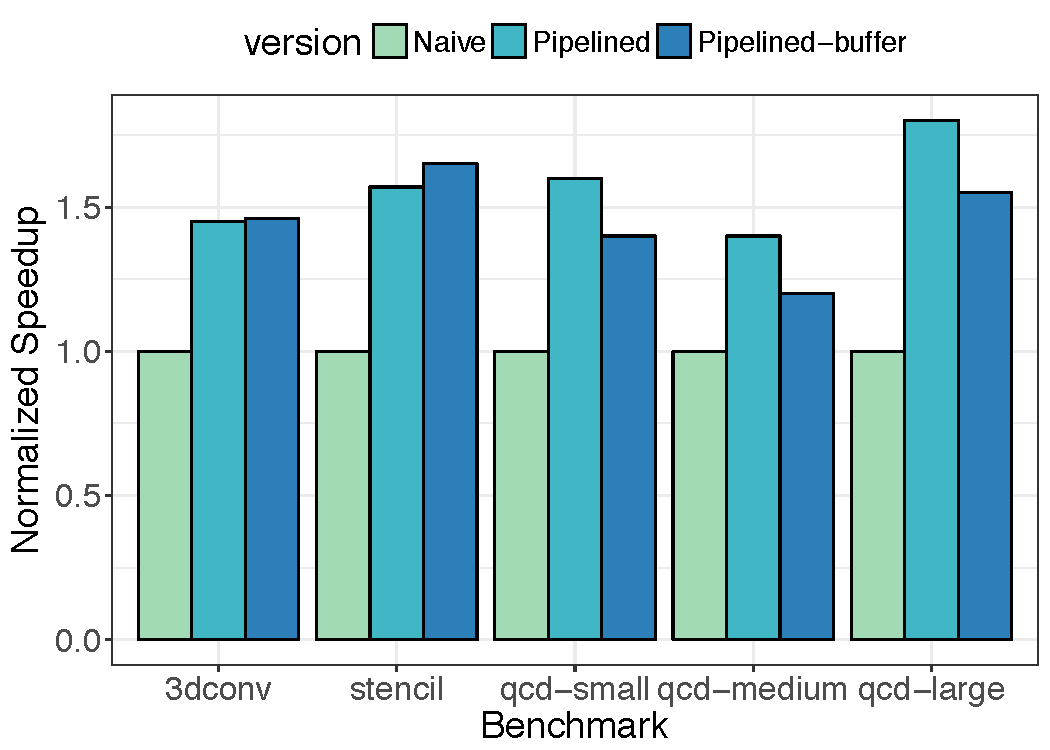
\includegraphics[width=0.5\textwidth]{pics/pipelining-perf}
  \caption{Speedup of pipelined or buffered data transfers across kernels.\label{pipeline-perf}}
\end{figure}


\subsection{Memory Affinity}
\label{sub:memory_affinity}

While OpenMP~5.0 will specify task affinity based on memory locations 
as discussed in Section~\ref{sub:new_tasking}, a longer term goal is to 
support more general memory affinity. Intuitive interfaces for this complex 
problem are difficult to specify. Nonetheless, we have explored interfaces
that associate data to computation and then appropriately locate, transform 
or replicate the data based on the distribution of the computation of existing
mechanisms in OpenMP~\cite{ctsar-tpds,scogland:7Hpt64iV}.
 
Figure~\ref{fig:atsar-gemm} shows a more recent direction that specifies how
to partition computation and to map the associated data range to the threads 
of a \texttt{parallel} region and then to a set of devices. This example 
partitions the GEMM loop into two-dimensional tiles by columns across sockets 
and rows across devices associated with a given socket. Extensions like this 
require careful consideration due to their potentially large number of changes,
and high complexity, but the information can support significant optimizations.
Beyond providing affinity information, these annotations are sufficient to 
allow for cross-device coscheduling across non-shared-memory devices.

Figure~\ref{fig:atsar-perf} shows performance results from a prototype 
implementation across five benchmark kernels in terms of speedup over a 
baseline OpenMP static schedule that uses all cores. The annotations and 
scheduling improvements that the information enables can increase performance 
substantially.  The optimization space being explored in the figure compares
static scheduling to an adaptive scheduler that attempts to predict the best 
partitioning based on past performance. The CPU adaptive results represent 
using the adaptive scheduler on the same resources as the baseline. The 
results also vary the devices across which the runtime system can 
distribute computation and data. It can use only the CPU cores, only a
set of one to four NVIDIA c1060 GPUs, or both. The same GEMM code can target
all of these options by changing runtime parameters.

The amount of expressive power this kind of extension can provide is
significant, but so is the complexity and the burden on the programmer who is
trying to use it.  We intend to continue exploring this space in the future to
provide an appropriate long-term solution.

\begin{figure}
  \begin{minted}[fontsize=\footnotesize]{c}
int i, is=0, ie=isz, j, js=0, je=jsz;
float A[ksz][jsz], B[isz][ksz];
float * C = (float*)malloc(sizeof(C[0])*isz*jsz);
int   C_pitch = jsz;

#pragma omp parallel devices(socket)              \
 part(adaptive: j_id=js; j_id<je; ++j_id)         \
 map(to: A[0:ksz][:,part=j_id], B[0:isz][0:ksz])  \
 map(tofrom: C[0:isz,pitch=C_pitch][:,part=j_id])
{ // Partitioned parallel region
#pragma omp target teams distribute parallel for  \
  devices(all) partition(dynamic)                 \
  map(to: A[:][:], B[:,partition=i][:])           \
  map(tofrom: C[:,partition=i][:])
  for (int i = is; i < ie; ++i) {//Partitioned loop
    for (int j = js; j < je; ++j) {
      float sum = 0.0;
      for (int k = 0; k < ksz; ++k) {
        sum += A[k][j] * B[i][k];
      }
      C[i * C_pitch + j] = sum;
    }
  }
}
\end{minted}
\caption{Possible Memory Affinity Interface\label{fig:atsar-gemm}}
\end{figure}

\begin{figure*}[t]
        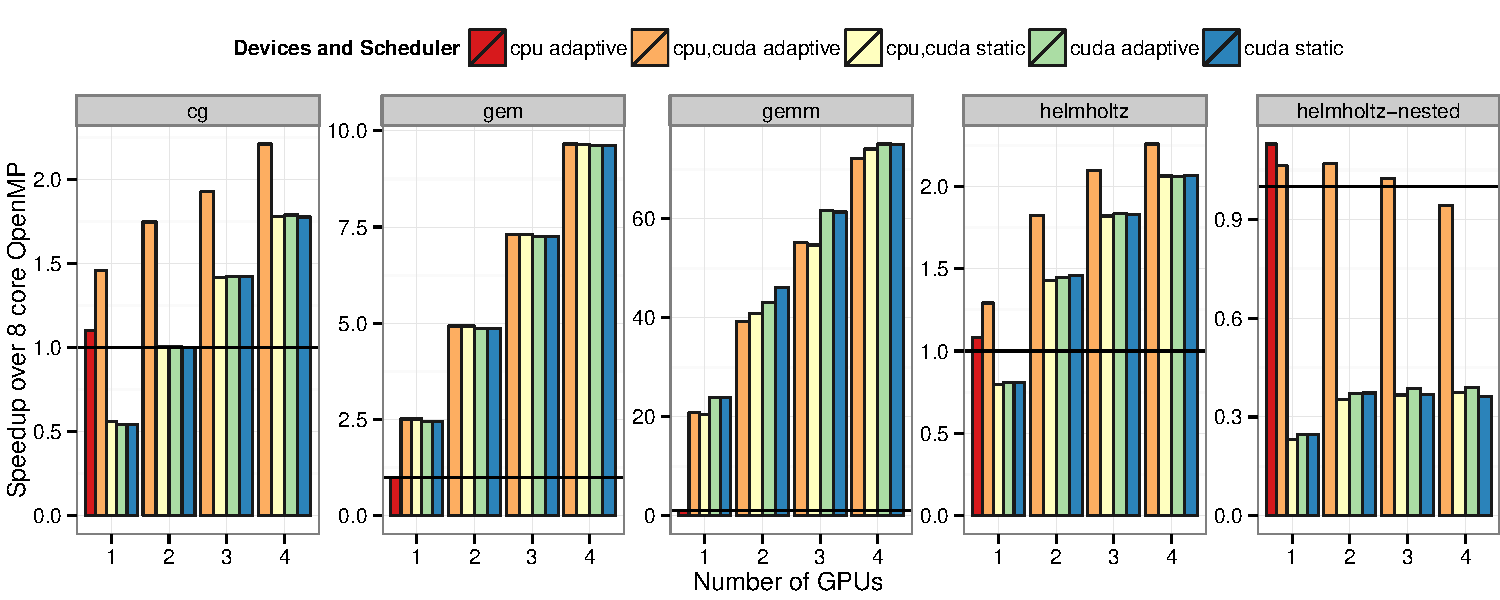
\includegraphics[width=\textwidth]{system-1-combined-part}
        \caption{Performance Benefit of Memory Partitioning/Affinity\label{fig:atsar-perf}}
\end{figure*}



\subsection{Free-Agent Threads}
\label{sub:task_only_threads}

%% BRONIS: This section would discuss the unshackled threads idea
%% BRONIS: I think I want to call them ``free-agent threads''

Currently, only threads of the parallel region in which an explicit
OpenMP task is generated can execute that task. This limitation leads
to the unintuitive (if simple) requirement that pure tasking programs 
in OpenMP must first start a \texttt{parallel} region and then must 
ensure that only one thread executes the code that generates the tasks, 
for example, by using a \texttt{single} region. This limitation can 
restrict parallelism in more complex applications since other threads 
(resources) may be idle and available to execute the tasks.

We are exploring a concept of free-agent threads to overcome this 
limitation. The mechanism would allow any thread that is not assigned
to a team to execute any explicit task. It would fully eliminate the
limitation -- all threads could execute explicit tasks that are 
generated in the initial thread without requiring an explicit 
\texttt{parallel} region. We need to resolve many details, such as
the return values for runtime routines such as \texttt{omp\_get\_thread\_num}
when executed by a thread that is not part of the team. Since this change 
will represent a major change in the OpenMP execution model, we do not 
expect to adopt it before OpenMP~6.0.





\subsection{Event-Based Parallel Programming Pattern}
\label{sub:concurrency_and_event_based_model}

One parallel programming pattern that OpenMP does not yet support is the
event-driven model that many interactive applications and networking servers
use. In this model, one or more threads run continuously in an event loop to 
observe external (e.g., user) actions. Other threads then perform the 
computation that the actions trigger to minimize response times. This 
event-based pattern naturally suits a task-based model. 
 
OpenMP's current task model does not suit the event-based pattern since it 
requires the team of the thread that generates a task to execute that task. 
To support this pattern, OpenMP needs a new capability to allow a thread to 
direct work toward a team other than its own. This capability would allow 
the event thread to remain responsive as other teams concurrently handle 
event processing. In addition, a mechanism that creates re-usable tasks 
could further improve response times. 


\subsection{Enabling Language-Level Outlining}
\label{sub:enabling_language_level_outlining}

As we discussed in Section~\ref{sub:outlining} outlining, or extraction 
of code into functions by the compiler, is one of the core mechanisms 
used to implement OpenMP. Some base languages provide outlining mechanisms 
in the form of closures or lambdas. The writers of libraries and parallel 
frameworks find these constructs attractive since they can describe abstract 
patterns and behaviors that then are passed an arbitrarily complex code 
sequence and associated data. Frameworks like Kokkos~\cite{kokkos} and 
RAJA~\cite{raja} exploit this mechanism to create flexible looping constructs, 
like the one in Figure~\ref{fig:raja}, that can be compiled for host devices, 
targets or any number of parallel backends depending on compile time arguments.
These mechanisms pose challenges to OpenMP, which OpenMP 5.0 will begin to
address.

\begin{figure}
\begin{minted}{c}
RAJA::forall<omp_parallel_for>(
    RAJA::range(0,N),
    [=](int a) {
      // loop body
});
\end{minted}
\caption{A \texttt{parallel for} Loop Body in a C++ Lambda}
\label{fig:raja}
\end{figure}
   
While OpenMP must evolve to support mechanisms such as lambdas, Fortran
users of OpenMP currently cannot exploit the capabilities that we will 
provide. So far, although many OpenMP implementations use outlining, they 
do not expose the resulting functions to the user. However, exposing these 
functions could provide many benefits, including a mechanism to support
closures in Fortran.
 
We could extend the \texttt{task} directive to create a form 
of "callable task" or OpenMP closure object that would be portable across 
C, C++ and Fortran. The extension would significantly reduce the work 
required to make an arbitrary callable object with state in C and Fortran.
It would also support library implementations with functionality like that 
of Kokkos and RAJA that all three languages could use. Challenges remain,
however, particularly how to integrate the functionality well into OpenMP 
and how to make it as efficient as possible at runtime. A simple and 
portable solution generates a structure, or derived type, and a function 
pointer. It would integrate well with established libraries, but is unlikely 
to optimize well for constructs that will be called many times. Despite 
the challenges, giving users control of outlining could be
a major step forward for OpenMP.







\section{Conclusion}
\label{sec:conclusion}

Over twenty years have passed since we released the first OpenMP specification.
It has become a mature programming API that continues to support Fortran, C, and
C++ as base languages. In its maturation, the size of the API and its
specification has grown substantially as we added support for additional
parallel programming patterns. Its underlying philosophy has also evolved
although we retain many of its core principles. Most of all, the primary purpose
of the API continues to be to allow users to specify information about their
computation that they easily know but that would require complex compiler
analysis to deduce while relying on the compiler to implement repetitive,
tedious and error-prone mechanisms that exploit that information in a way that
can be carried from compiler to compiler.  As of this writing, there are sixteen
compilers listed on the OpenMP compilers page~\cite{openmp-compilers}, with nine
of them supporting at least a significant portion of OpenMP 4.5.

In this paper, we discussed the $7.5\times$ increase in the size of the 
OpenMP specification over the course of its lifetime. We provided 
a glimpse into the evolution of its guiding principles as well as
some of the features that the most recent versions added. We also
discussed some of the key programming features that OpenMP 5.0 will
add and that are under consideration for versions beyond it. These
plans will result in a specification that supports essentially every 
major parallel programming pattern and the latest base language standards.



% \section*{Acknowledgments}

%% TODO: Michael needs to check what parts of these disclaimers will actually be needed and what we can remove
* Other names and brands are the property of their respective owners.

Software and workloads used in performance tests may have been
optimized for performance only on Intel microprocessors.  Performance
tests, such as SYSmark and MobileMark, are measured using specific
computer systems, components, software, operations and functions.  Any
change to any of those factors may cause the results to vary.  You
should consult other information and performance tests to assist you
in fully evaluating your contemplated purchases, including the
performance of that product when combined with other products.  For
more information go to \url{http://www.intel.com/performance}.

Intel's compilers may or may not optimize to the same degree for
non-Intel microprocessors for optimizations that are not unique to
Intel microprocessors. These optimizations include SSE2, SSE3, and
SSSE3 instruction sets and other optimizations. Intel does not
guarantee the availability, functionality, or effectiveness of any
optimization on microprocessors not manufactured by
Intel. Microprocessor-dependent optimizations in this product are
intended for use with Intel microprocessors. Certain optimizations not
specific to Intel microarchitecture are reserved for Intel
microprocessors. Please refer to the applicable product User and
Reference Guides for more information regarding the specific
instruction sets covered by this notice.

% usual LLNL boilerplate
This work was performed under the auspices of the U.S. Department of Energy by
Lawrence Livermore National Laboratory under Contract DE-AC52-07NA27344.

% Stephen: Must have the SNL ack if I am on the paper:

Sandia National Laboratories is a multimission laboratory managed
and operated by National Technology and Engineering Solutions of
Sandia, LLC., a wholly owned subsidiary of Honeywell International,
Inc., for the U.S. Department of Energy's National Nuclear Security
Administration under contract DE-NA-0003525.



\begin{spacing}{0.9}
  \bibliographystyle{abbrv}
  % \balance
  \bibliography{bib/tom-papers}
\end{spacing}

% BIOS START HERE: currently disabled

% \graphicspath{{authors/}}
%
% {\footnotesize
% \begin{IEEEbiography}[{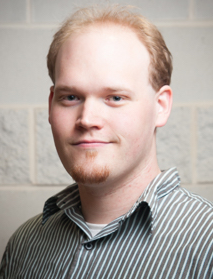
\includegraphics[width=1in,height=1.25in,clip,keepaspectratio]{tom}}]{Thomas R.W. Scogland}
received his PhD degree in computer science from Virginia Tech in 2014.  He is a
computer scientist in the Center for Applied Scientific Computing at Lawrence
Livermore National Laboratory. His research interests include parallel
programming models, heterogeneous computing and resource management at scale.
He serves on the OpenMP Language Committee, the C and C++ committees, and as
co-chair of the Green500.
\end{IEEEbiography}


% \vfill
% \input{authors/wu.tex}
% \vfill
% \input{authors/barry.tex}
% \vfill
% \begin{IEEEbiography}[{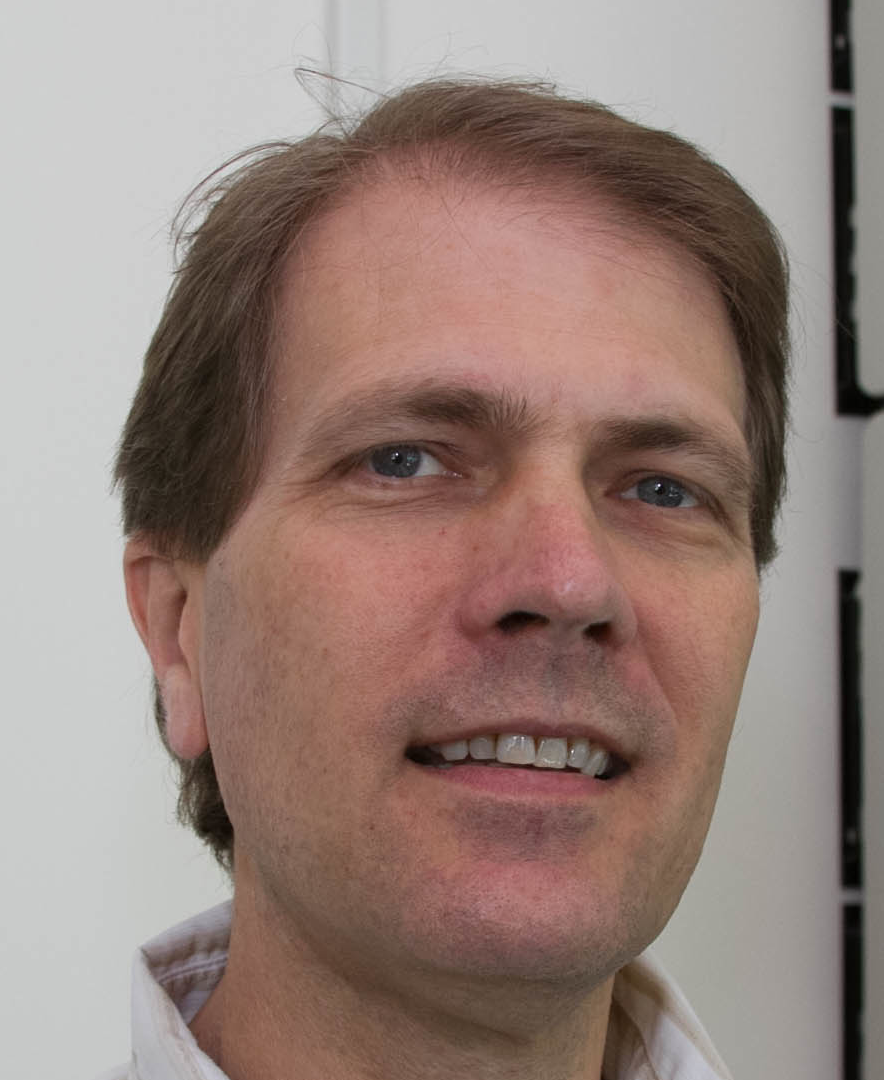
\includegraphics[width=1in,height=1.25in,clip,keepaspectratio]{bronis.cropped}}]{Bronis R. de~Supinski}
is the Chief Technology Officer (CTO) for Livermore Computing (LC) at 
Lawrence Livermore National Laboratory (LLNL). In this role, he
formulates LLNL's large-scale computing strategy and oversees its 
implementation. He earned his Ph.D. in Computer Science from the University 
of Virginia in 1998 and he joined LLNL in July 1998. In addition to his work 
with LLNL, Bronis is also a Professor of Exascale Computing at Queen's 
University of Belfast and an Adjunct Associate Professor in the Department 
of Computer Science and Engineering at Texas A&M University. Throughout his 
career, Bronis has won several awards, including the prestigious Gordon Bell 
Prize in 2005 and 2006, as well as an R&D 100 for his leadership in the
development of a novel scalable debugging tool.
\end{IEEEbiography}


% }

% BIOS END HERE

\end{document}
